\chapter{Appendix}

\ifpdf
    \graphicspath{{Appendix/AppendixFigs/PNG/}{Appendix/AppendixFigs/PDF/}{Appendix/AppendixFigs/}}
\else
    \graphicspath{{Appendix/AppendixFigs/EPS/}{Appendix/AppendixFigs/}}
\fi

  \begin{figure}[!htpb]
      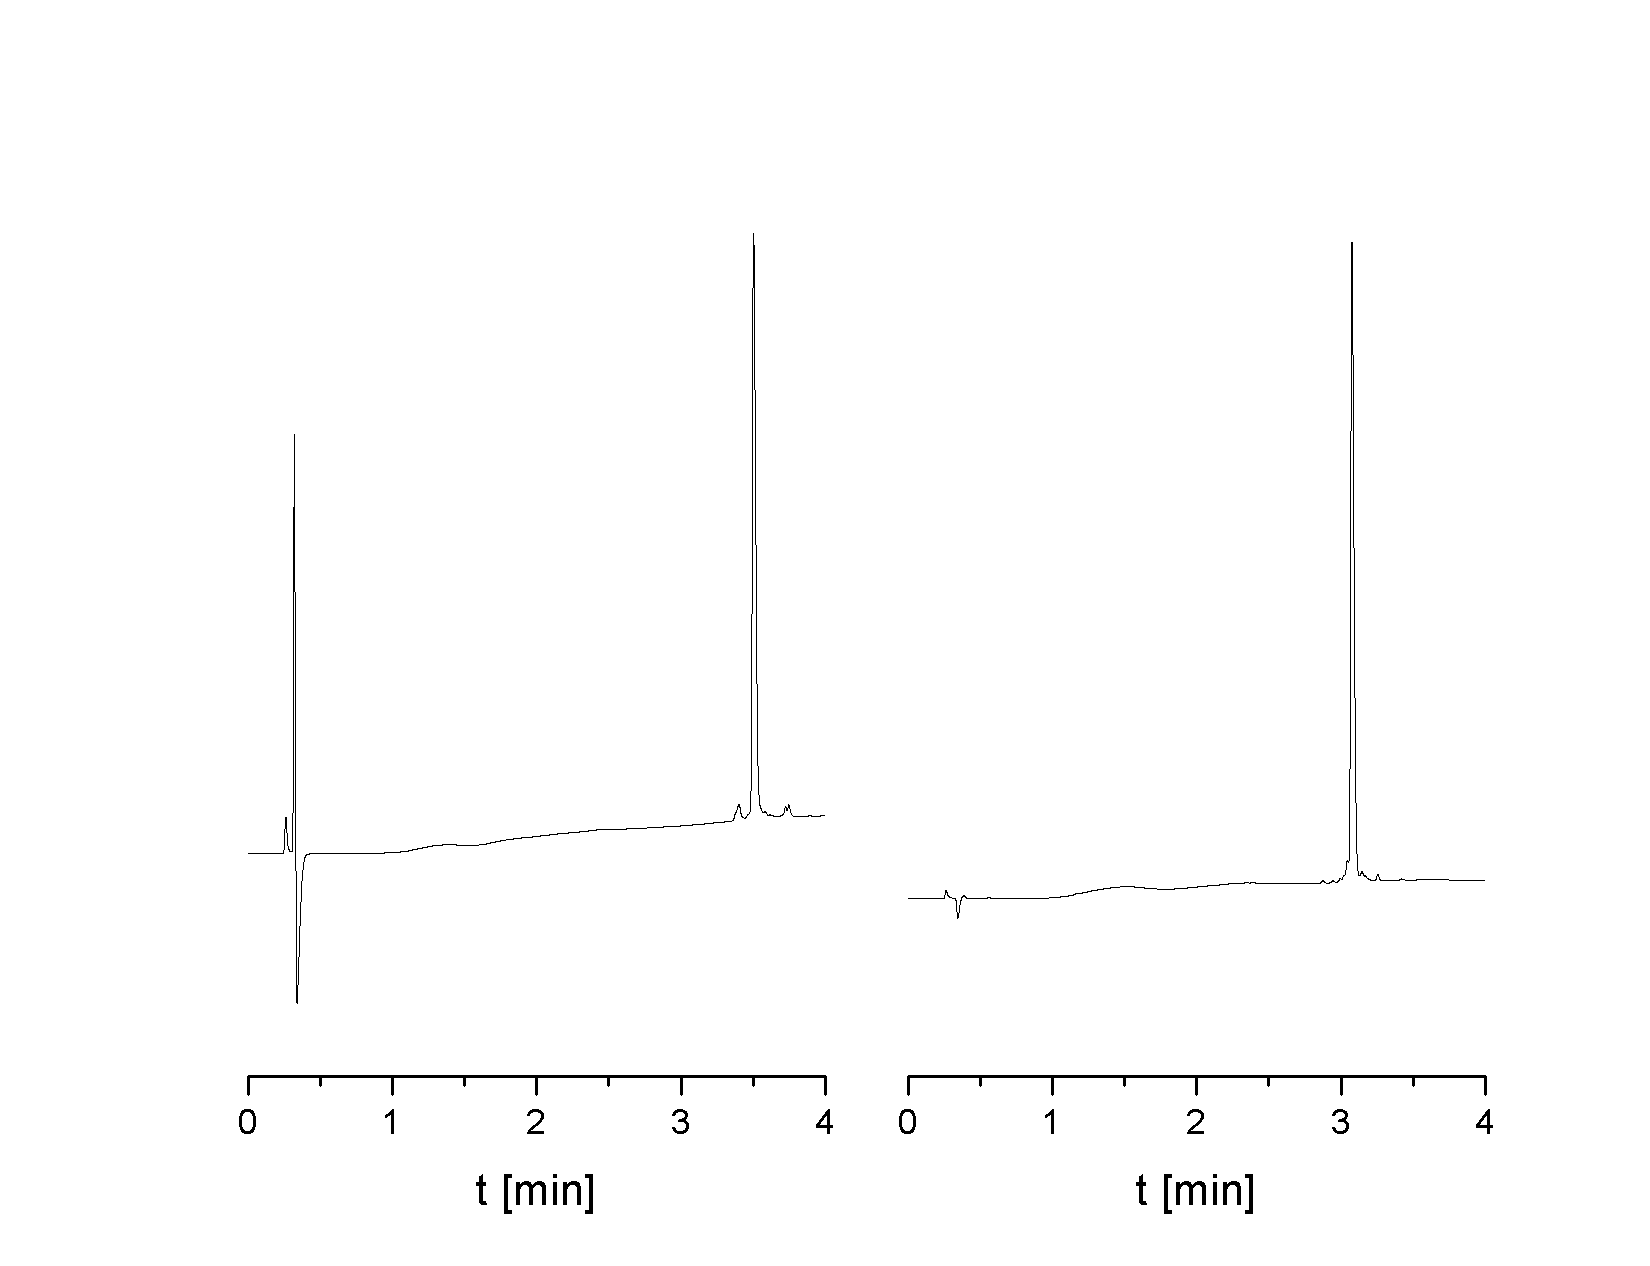
\includegraphics[width=\textwidth]{MeoBrAuxPeps.png}
      \caption{UPLC trace of 4-bromophenyl (\cmpd+{cmpd:auxiliarypeptide.one}) and 4-methoxyphenyl (\cmpd+{cmpd:auxiliarypeptide.two}) auxiliary peptides}
      \label{fig:auxpepuplc}
  \end{figure}

\begin{figure}
    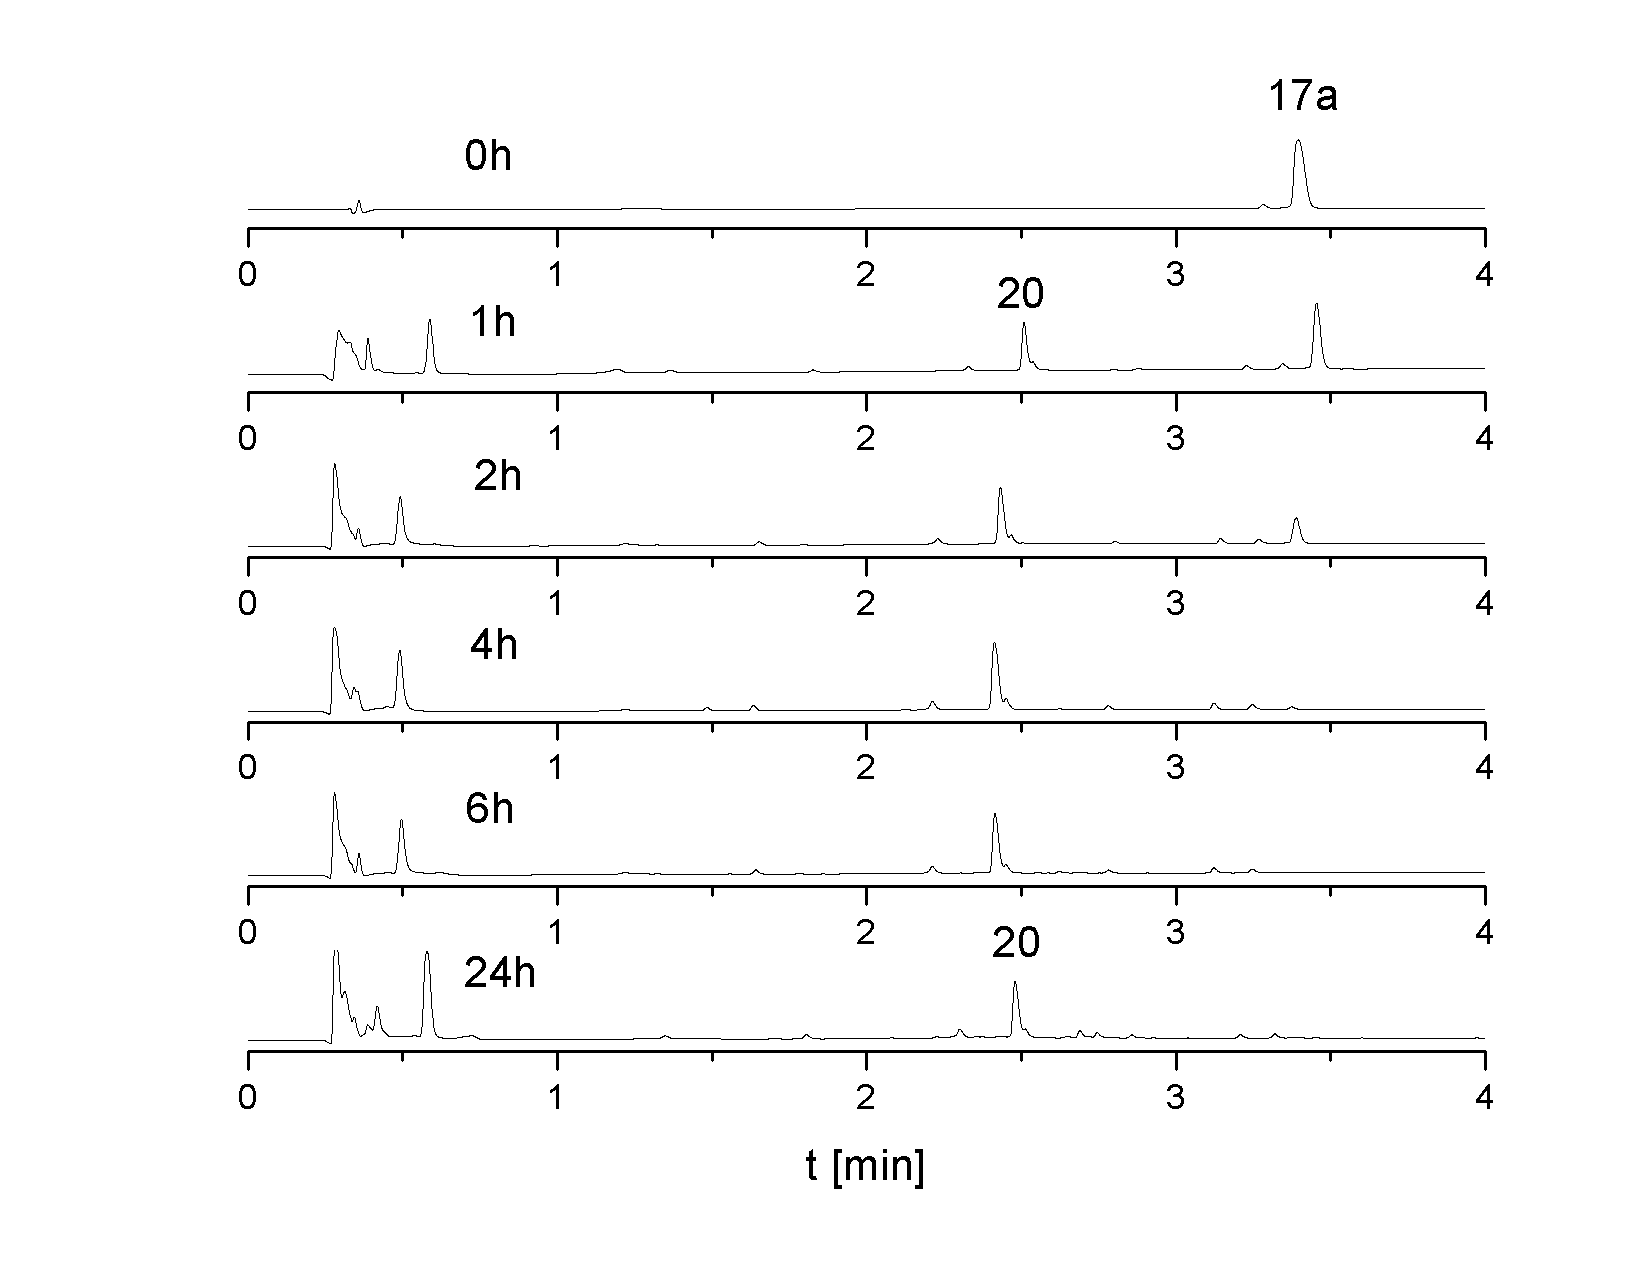
\includegraphics[max width=\linewidth]{br50cleavage.png}
    \caption{UPLC trace for the cleavage of \cmpd+{cmpd:auxiliarydipeptide.one} (100 mM TCEP, \SI{50}{\celsius})}
    \label{fig:br50cleave100}
\end{figure}

\begin{figure}
    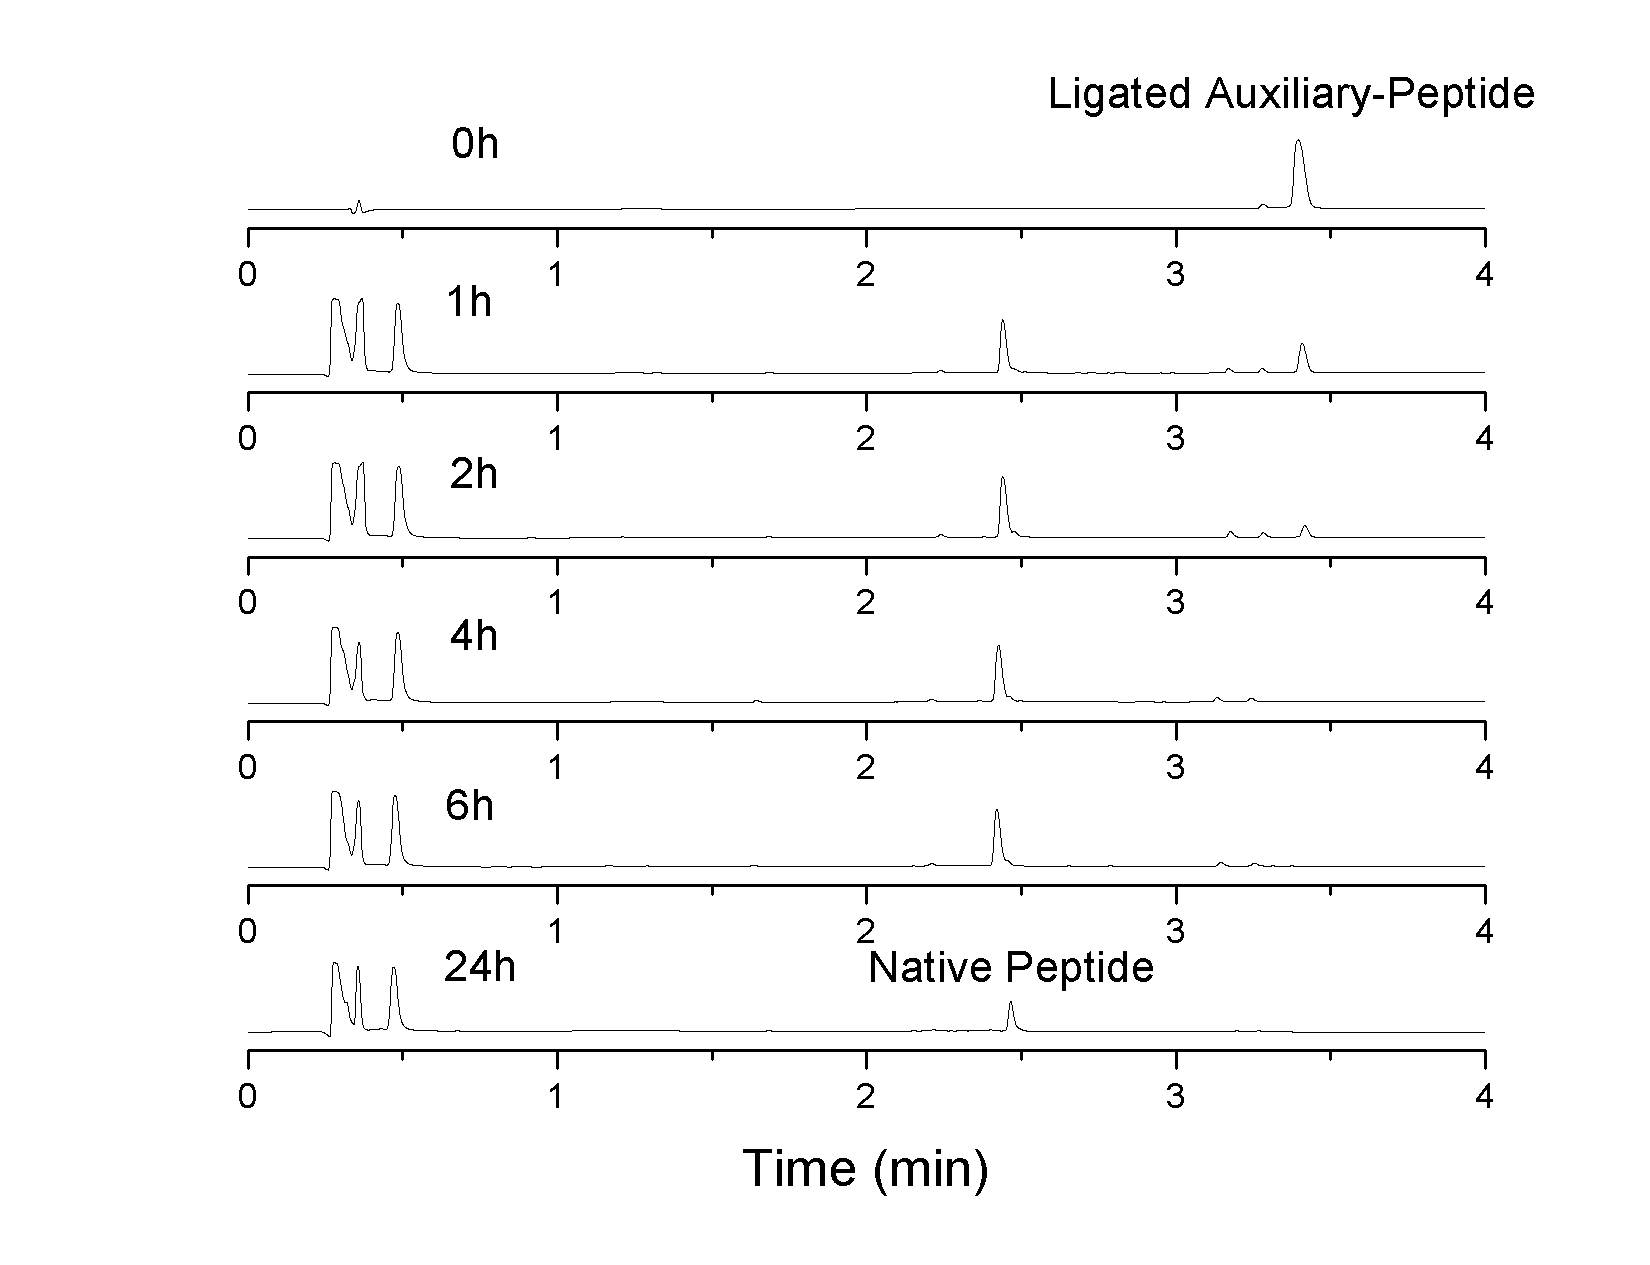
\includegraphics[max width=\linewidth]{brrtcleavage.png}
    \caption{UPLC trace for the cleavage of \cmpd+{cmpd:auxiliarydipeptide.one} (400 mM TCEP, R.T.)}
    \label{fig:brrtcleavage}
\end{figure}

\begin{figure}
    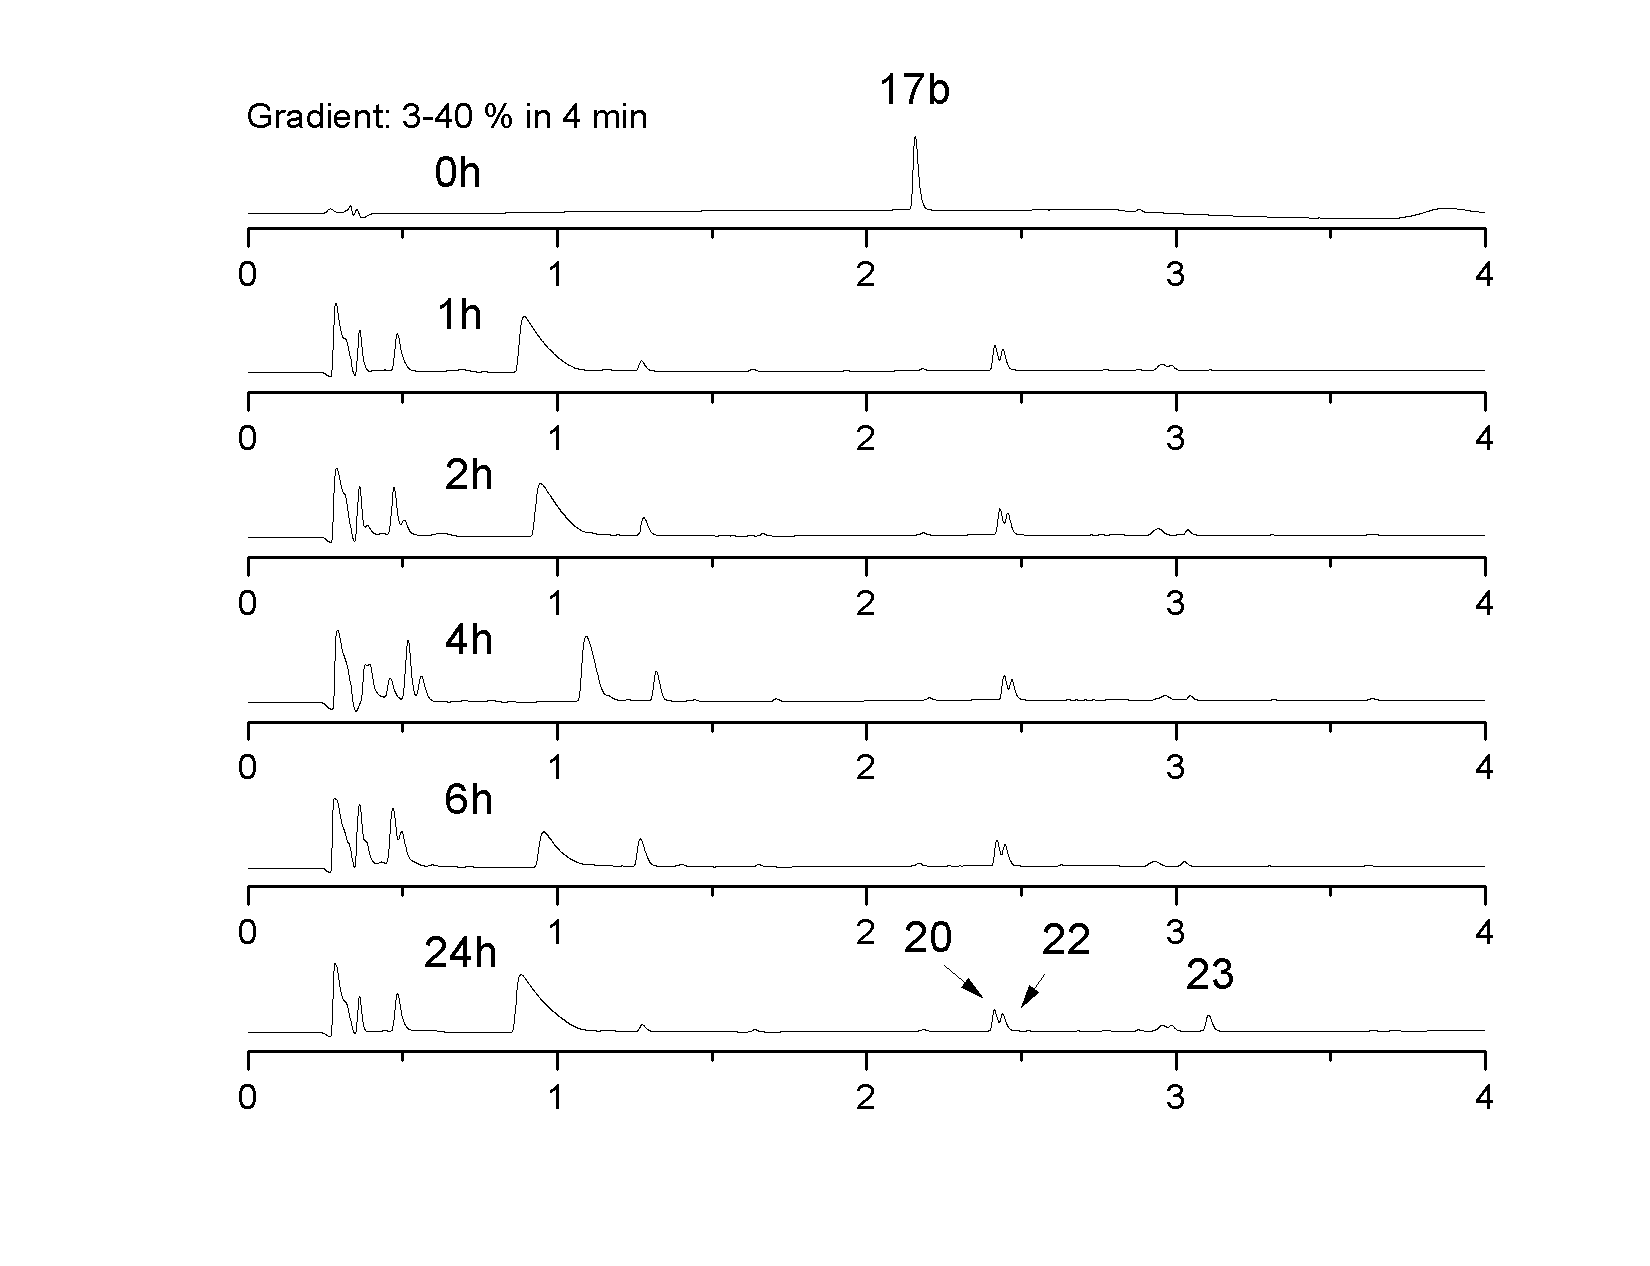
\includegraphics[max width=\linewidth]{meoinitiatorcleavage.png}
    \caption{Side product formation during cleavage of \cmpd+{cmpd:auxiliarydipeptide.two} in the presence of a radical initator (VA-044 20 eq.)}
    \label{fig:meoinitatorcleavage}
\end{figure}

\begin{figure}
    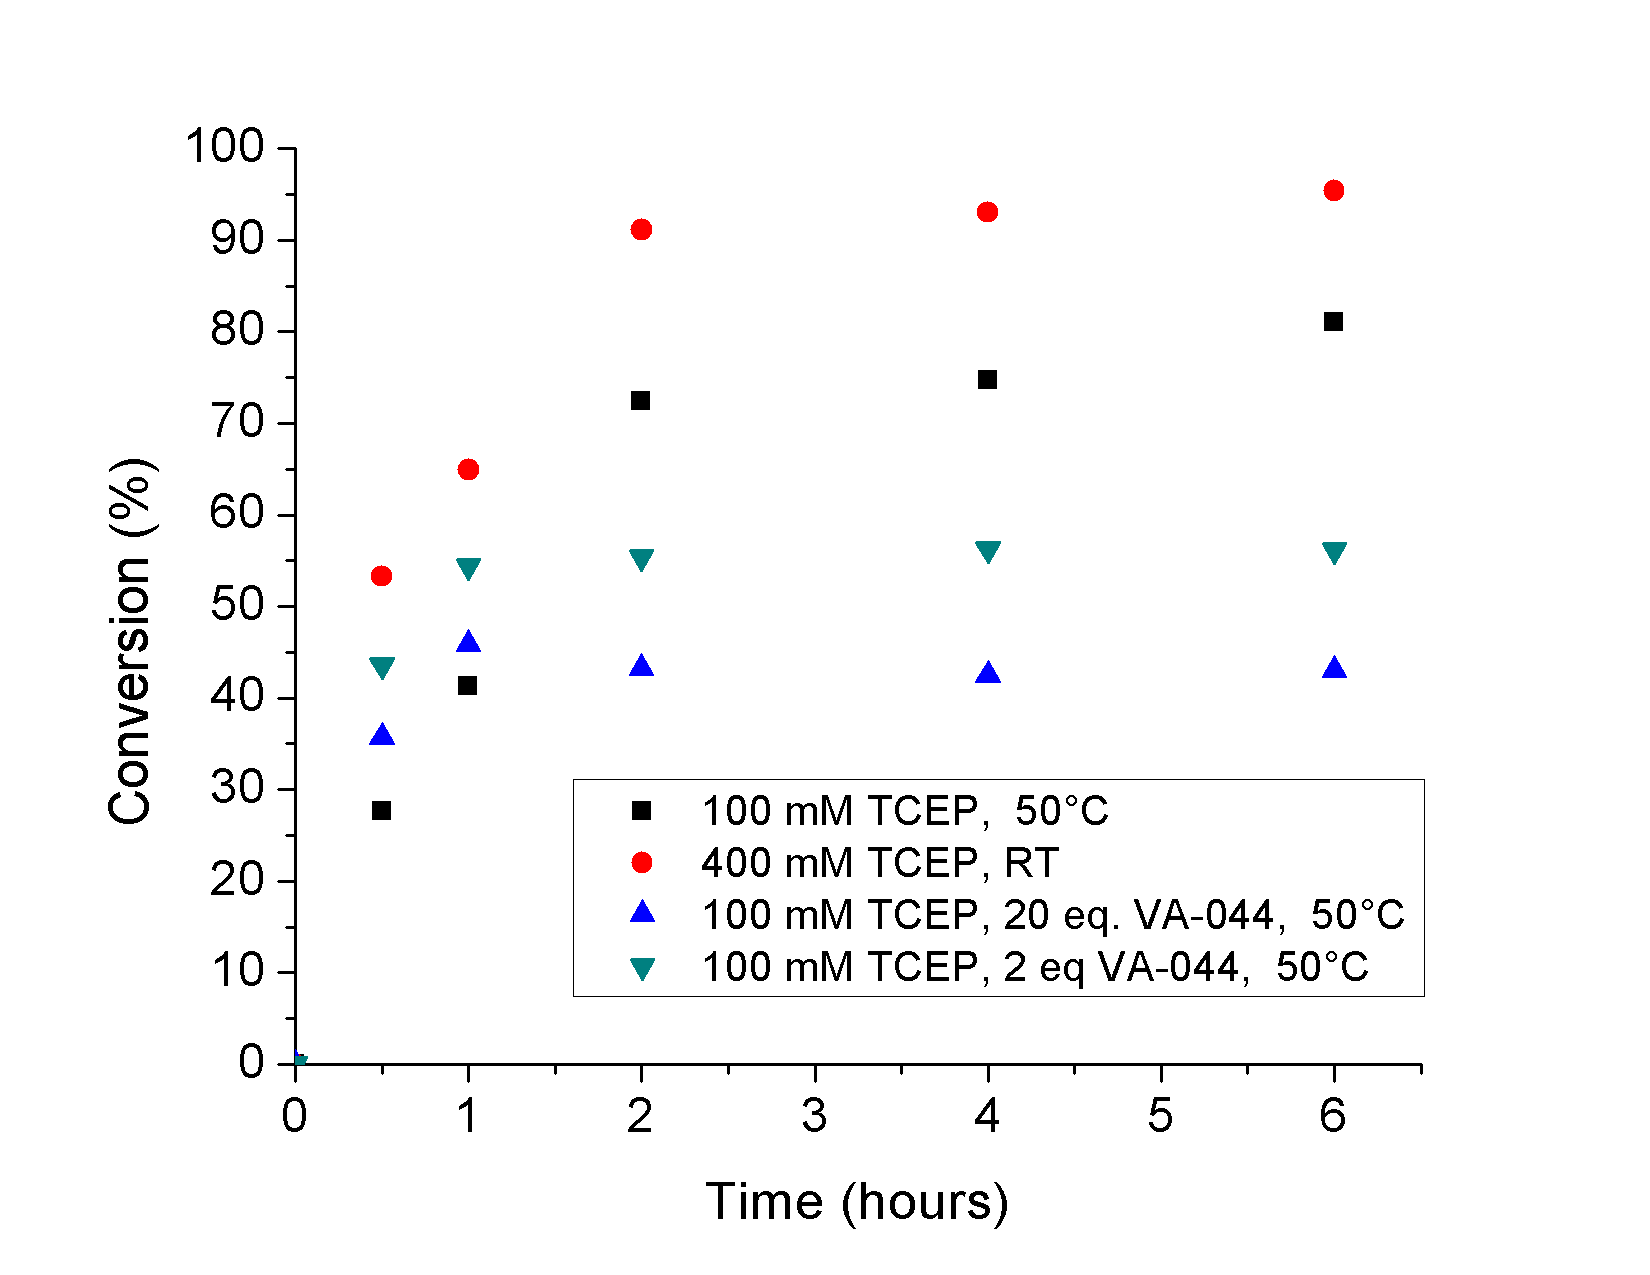
\includegraphics[max width=\linewidth]{meocleavage.png}
    \caption{Rate of auxiliary peptide \cmpd+{cmpd:auxiliarydipeptide.two} cleavage}
    \label{fig:meocleavagerate}
\end{figure}
% ------------------------------------------------------------------------

%%% Local Variables:
%%% mode: latex
%%% TeX-master: "../thesis"
%%% End:
